\documentclass[]{article}
\usepackage{graphicx}
\usepackage{hyperref}
\usepackage{amsmath}
\usepackage{caption}
\usepackage{subcaption}
\usepackage[utf8]{inputenc}
\usepackage{float}

%opening
\title{Saturated Absorption Spectroscopy for the $D2$ lines of $^{87}Rb$ and $^{85}Rb$ at room temperature }
\author{Gunther T\"urk, Jonas Lehnen}

\begin{document}

\maketitle
\begin{abstract}
The comparison of saturated and normal absorption spectroscopy leads to the confirmation of better resolution regarding the hyperfine structure.  
By measuring the $D2$ lines of $^{85}Rb$ and $^{87}Rb$, in a ratio of $72.2 : 27.8$, we were able to confirm the relative frequencies of the energy levels. Additionally the expected room temperature for the rubidium gas has been confirmed.
\end{abstract}

\newpage
\tableofcontents



\newpage
\section{Introduction}
Understanding the behaviour of excited atomic states and being able to manipulate them is a part of atomic physics. To visualize the energy transitions a spectrum has to be taken and analysed. 
This experiment about laser spectroscopy will show the problem of absorption spectroscopy (AS) regarding the resolution of the transitions energy. This will be shown at the example of $^{87}Rb$ and $^{85}Rb$. The transition between $5^2S_{1/2}$ and $5^2P_{3/2}$, also called $D2$ line, will be excited with a $780nm$ laser. The natural linewidth of this transition is $\Gamma = 2\pi \cdot 5.8\ MHz$.
Due to Doppler broadening an atom can be excited in a wider range of energy, thereby it is not possible to resolve the hyperfine structure. The application of saturated absorption spectroscopy (SAS) will improve the spectrum to shown the exact transitions within the Doppler broadening. With the comparison to the theoretical values a confirmation for the hyperfine structure will be possible.

The Doppler broadening spectrum itself is not useless and contains information about the temperature of the material. Therefore an estimation is possible and can be compared to the room temperature to see the effects of the driven excitations on the material.



\newpage
\section{Theory}
\subsection{Absorption spectroscopy}
The transmitted intensity of light after the transition through matter can be described with the Lambert Beer law. The transmission $T$ depends on the materials length $L$ and the absorption coefficient $\alpha$ which is depending on the resonance frequency $\omega_0$ of the individual atomic transitions as well the natural linewidth $\Gamma$ of this transition.

\begin{equation}
T(\omega)\approx 1-\alpha(\omega)L \:,\: \alpha(\omega)= \alpha(\omega_0)\frac{\Gamma/2\pi}{(\omega-\omega_0)^2 + (\Gamma/2\pi)^2}
\end{equation}

This results in a valley in the intensity for each $\omega_0$ the laser stimulates, due to the maximum in absorption. Each minimum should be formed like a Lorentzian, due to the prportionality in $\alpha$. For fitting this curve is not useful, because a standard derivation is not properly defined. 

\subsection{Doppler broadening}
The natural linewidth $\Gamma$ describes for which frequency around $\omega_0$ the transition can be driven. This is equal to the full width at half of the maximum (FWHM) $\delta\omega_{Natural} = \Gamma$. For a Gaussian the relation $FWHM = 2 \sqrt{2ln(2)} \sigma$ is used.

Now the Doppler effect is able to increase this range of frequencies depending on the atoms velocities relative to the incoming photons. Thereby their frequency is increased when moving towards each other and decreased in the case of moving in the same direction. For the first case, this mean a photon with $\omega < \omega_0$ can already excite the atom. And thereby the range of exciting frequencies is increased. This is described by \autoref{dopplershift} where $\vec{k}$ and $\vec{v}$ are the wave vector of the photon and the velocity of the atom.

\begin{equation}
\omega  = \omega_0 + \vec{k}\vec{v} = \omega_0 \left(1+\frac{v_{||}}{c} \right)\:,\: c = \omega_0\cdot |\vec{k}|
\label{eq:dopplershift}
\end{equation}

For a system in thermal equilibrium the velocity distribution for $v_{||}$, in direction of the photons, is given by the the Maxwell-Boltzmann distribution for N particles. 

\begin{equation}
n(v_{||})dv_{||} = \frac{N}{v_W \cdot \sqrt{\pi}} exp\left[ - \frac{v_{||}^2}{v_W^2} \right] dv_{||} \:,\: v_W= \sqrt{\frac{2k_BT}{m}}
\end{equation}

This includes the mass of the atoms m as well as the temperature T of the whole system. The transmitted intensity is directly proportional to $n(v_{||}) dv_{||}$, because this returns the atoms which are able to drive the excitation. Rewriting $v_{||}$ with \autoref{eq:dopplershift} we end up with a Gaussian for each $\omega_0$ in our spectrum of the Doppler broadening.

\begin{equation}
I(\omega)=I(\omega_0)\ exp\left[ - \frac{(\omega-\omega_0)^2}{\omega_0v_{||}\ / c}\right] \:,\: \delta\omega_{Doppler} = 2 \sqrt{ln(2)} \cdot \omega_0\frac{v_W}{c}
\label{eq:gauss}
\end{equation}

For room temperature $T=300K$ this results in $\delta\omega_{D} \approx 3201\ MHz$. Compared to the usual hyperfine transitions for the excited state in \autoref{fig:Rb_hyperfine}, this value is too high to resolve those transitions. Therefore a different approach has to be made.

\subsection{Saturated absorption spectroscopy}
Instead of using only one laser the idea of SAS is to split it and make use of the atoms velocity distribution. The laser is split in a pump beam with higher intensity than the other probe beam. They will be send through the atoms from different sides. Thereby each one will mostly excite the atoms according to \autoref{eq:dopplershift}. The probe beams intensity will be measured. If the lasers frequency is exactly on resonance, spectral hole burning of the pump beam can be observed. This means the maximum of 50\% of the atoms will be excited. Therefore the probe beam won't be able to excite any atoms, and therefore won't lose its intensity. Instead due to stimulated emission the intensity it will be increased. This is called "lamb dip", due to break down in the probe beams absorption, but a peak in intensity will be observed. On this way the individual peaks of the hyperfine transitions will be resolved.

\subsection{Cross over resonances}
In the spectrum of SAS additional peaks will be observable. They are created when the lasers frequency is exactly between two transitions. For example, the pump beam will excite the transition $\hbar\omega_{01}$ with atoms moving with $+v_{||}$ and simultaneously $\hbar\omega_{02}$ with $-v_{||}$. The probe beam, coming from the other spacial direction, will try to excite $\hbar\omega_{01}$ with $-v_{||}$ and $\hbar\omega_{02}$ with $+v_{||}$, the exact opposite velocities. Because of the already excited atoms, for the probe beam the medium becomes transperent again and an additional peak will be visible.

\begin{equation}
\omega_{CO 12} = \frac{\omega_{01}+\omega_{02}}{2}
\end{equation}

\subsection{Rubidium}
In this experiment rubidium is used. The reason is that the transitions between $5^2S_{1/2} \rightarrow 5^2P_{3/2}$ is at around $780nm$ which is a good wavelength to build laser for. The other reason is that the hyperfine structure for the two isotopes $^{87}Rb$ and $^{85}Rb$ is exactly the same regarding the structure and not the energy itself. The different shifts in energy are mostly caused by the different nucleus spins: $I(^{87}Rb)=\frac{3}{2}$ and $I(^{85}Rb)=\frac{5}{2}$. The relation is shown in \autoref{eq:HFS} where $\mu_K$ is the magnetic moment of the nucleus, $g_I$ is the Landé factor for nucleus spin coupling and $B_j$ the magnetic field induced by the coupling of spin and orbit, see \cite{dem3}.

\begin{equation}
\Delta E_{HFS}=\frac{A}{2} [F(F+1) + j(j+1) - I(I+1)] \;,\;\; A= \frac{g_I \mu_K |B_j|}{\sqrt{j(j+1)}}
\label{eq:HFS}
\end{equation}



\newpage
\section{Experimental set-up}
\begin{figure}[H]
\centering
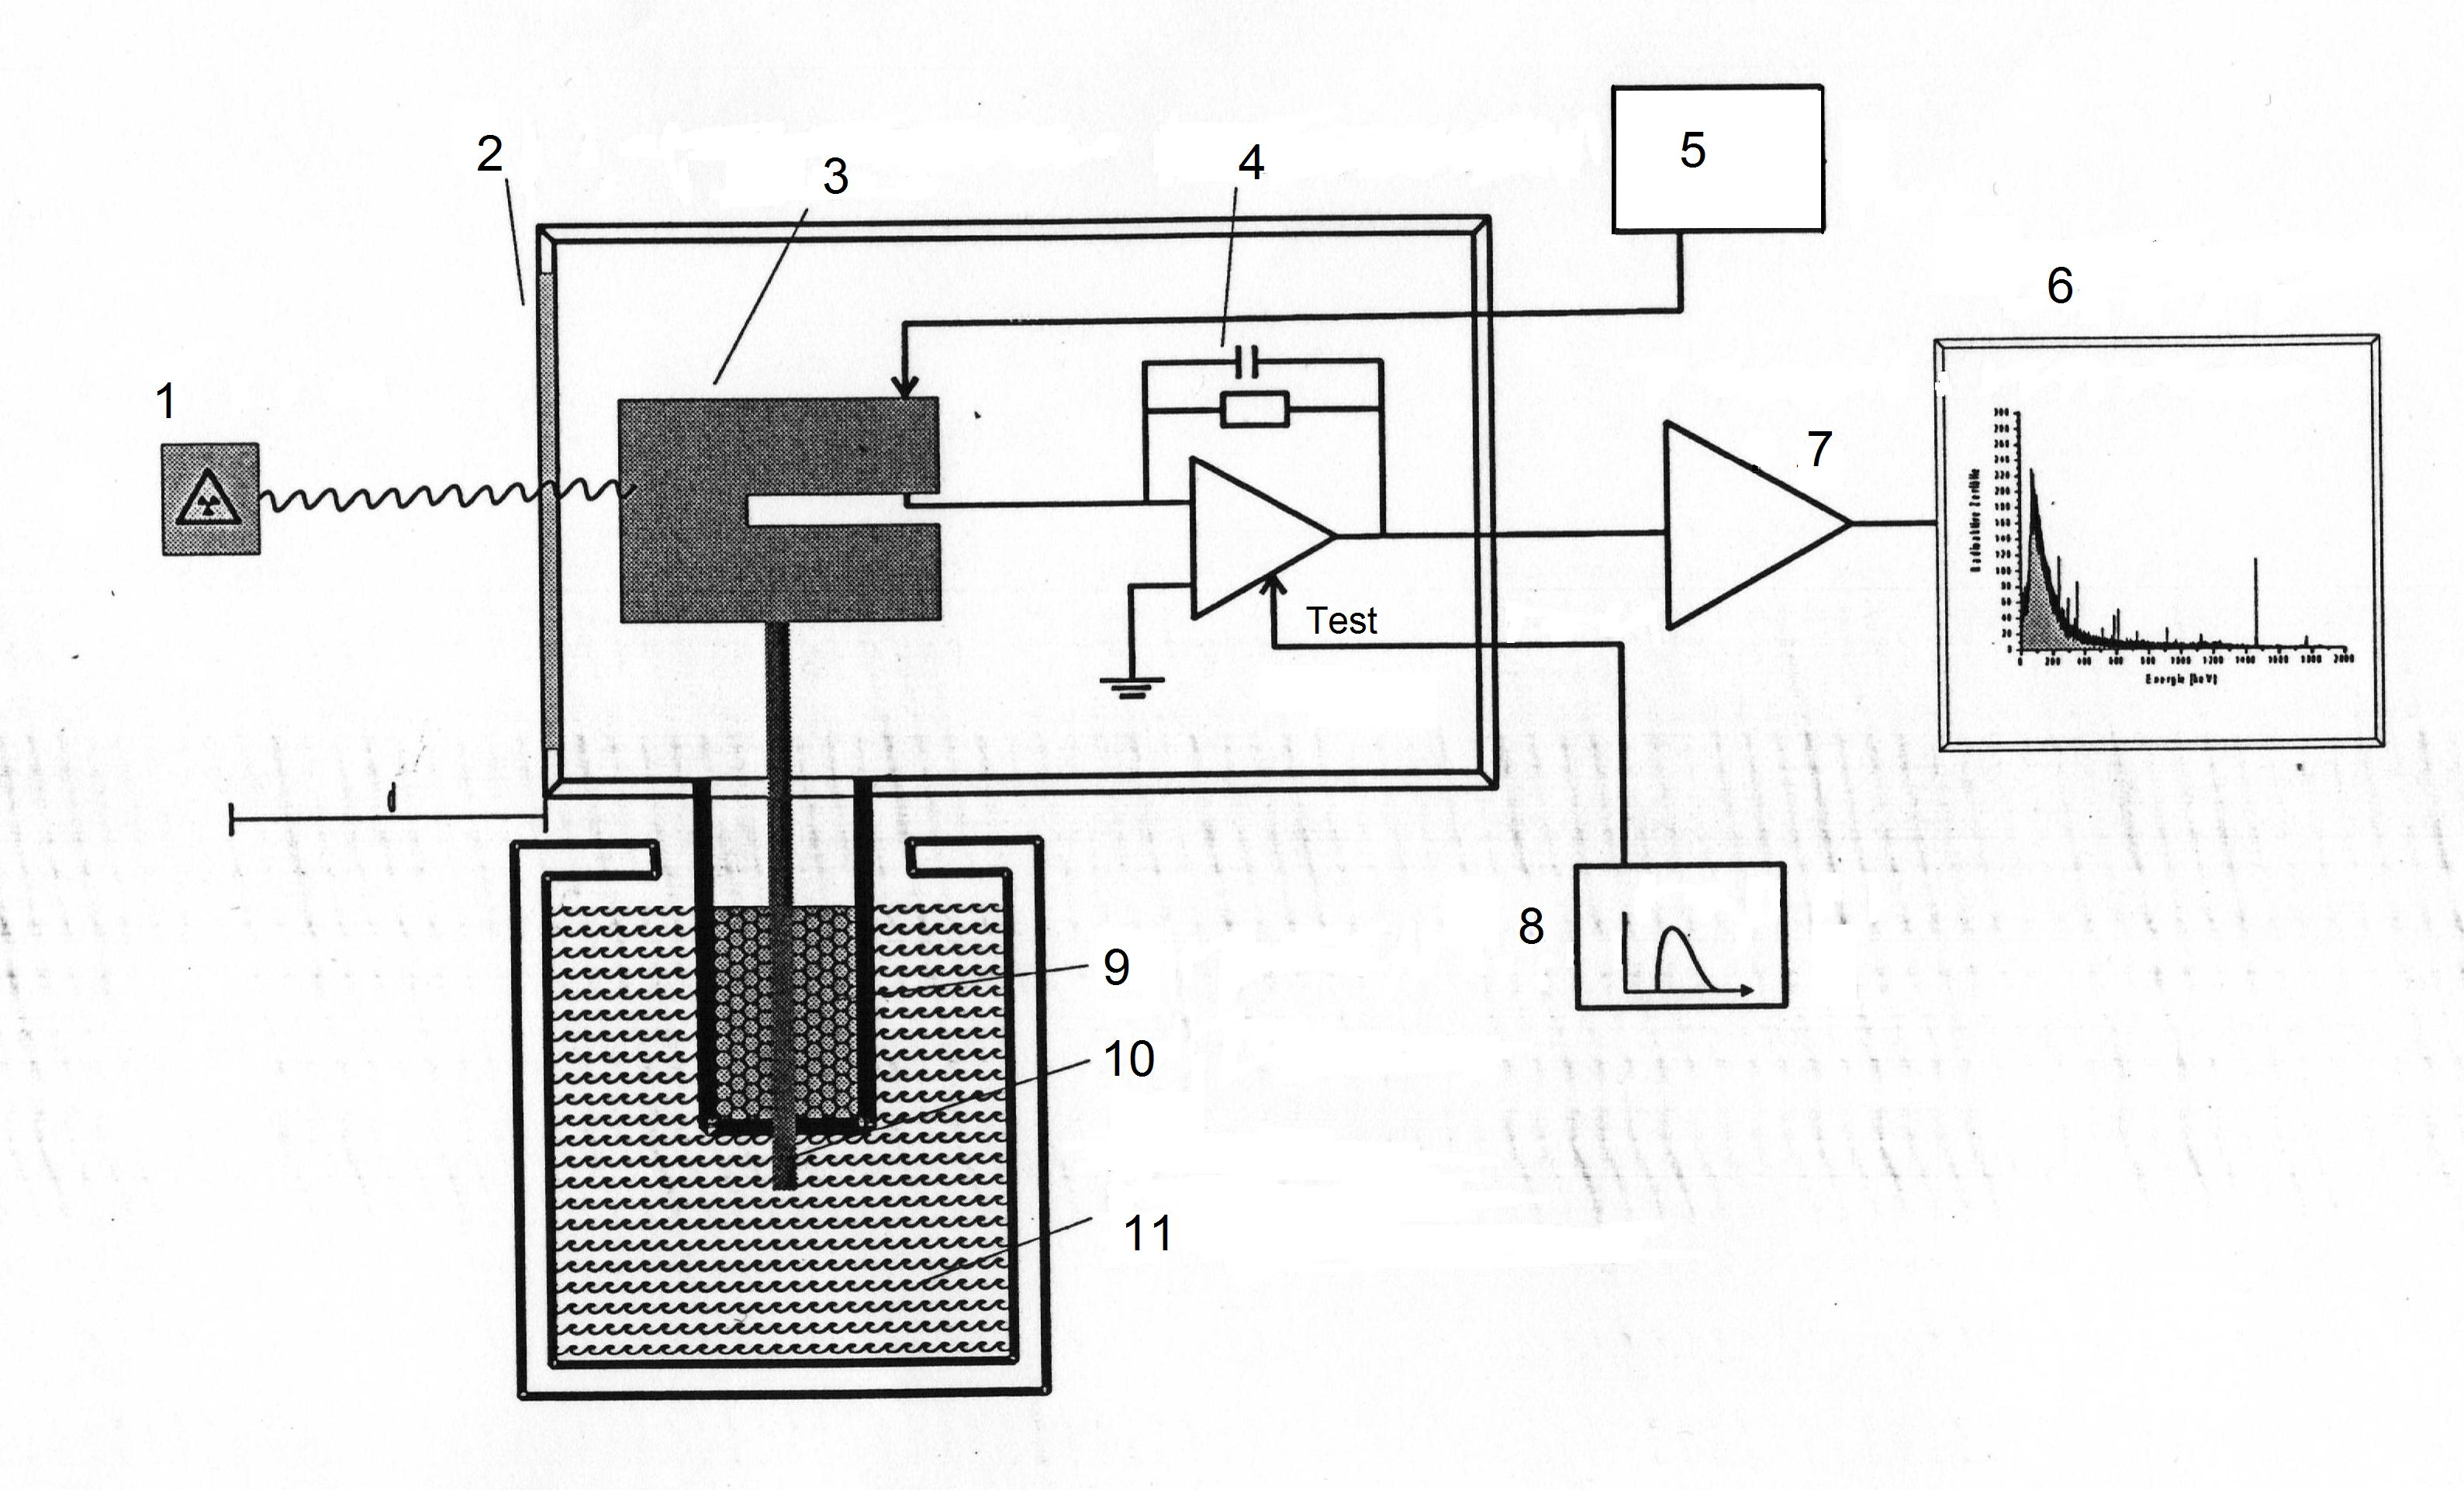
\includegraphics[width=1\textwidth]{Plots/Setup.png}
\caption{Schematics of the experimental set-up used.}
\label{fig:setup}
\end{figure}

For this experiment a rubidium gas cell of the isotopes $^{85}Rb$ and $^{87}Rb$ with an ratio of $72.2 : 27.8$ is used. The wavelength of the laser was set on $780.24nm$. As shown in \autoref{fig:setup} the laser is split by the polarising beam splitter. The distribution of the polarisations is regualted in advance with the $\lambda/2$ wave-plate. Because we don't know which polarisation is favoured by the laser we adjust the wave-plate in such a way, that the pump beam has the significant higher intensity. This can be monitored by intersecting the laser with a piece of paper. Important is to overlap both beam while they are in the gas cell to prevent intensity-loss of the probe beam on resonance.

Setting the laser is the difficult part of this experiment. You have to find a spectrum without mode hops. This mean that for all time the same wavelength is standing in your laser cavity. For small changes in current or temperature, the wavelength can change and a different spectrum will be visible. A small triangular ramp signal will be added to the laser currents fine adjustment by a piezoelement to screen different frequencies. For the calibration another signal generator is used to create sidebands, see \autoref{fig:all}.

In the end a photo diode will register the probe beams intensity. In our case the signal will be visualized by an oscilloscope and from there data will be recorded via an USB stick.



\newpage
\section{Analysis}
\subsection{Spectrum}
\begin{figure}[H]
\centering
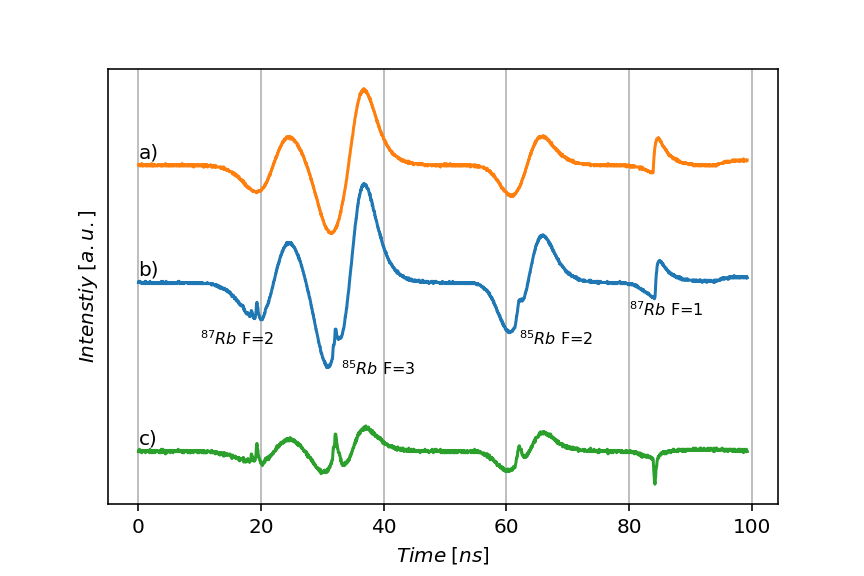
\includegraphics[width=.8\textwidth]{Plots/Diff_Signal.png}
\caption{Spectrum of the rubidium gas cell. a) AS, b) SAS, c) Difference signal}
\label{fig:signals}
\end{figure}

As shown in \autoref{fig:signals} the difference between the spectra of the different methodes are grave. As expected a) shows no hyperfine transitions due to insufficent resolution. For b) those are now clearly visible and will be used to identify the transitions in the following chapters. They are already labelled according to the transitions shown in \ref{fig:Rb_hyperfine}.
The difference signal c) should only show the peaks of the hyperfine structure.
Usually the difference signal should show no sign of any remains of the Doppler broadening signal. It seems as there are some fluctuations caused by the second laser, because the Doppler broadening is higher for the SAS. 

For the last peak  $^{87}Rb\ F=1$ the difference is not correctly calculated. There shouldn't be such a strong dip in the signal. This is probably caused by the very few data values the oscilloscope saved in this region. The fast rise consists of less than 10 values and is therefore a bad example to argue with. This problem will occur later for the estimation of the rubidium gas temperature.


\subsection{Calibration}
\begin{figure}[H]
\centering
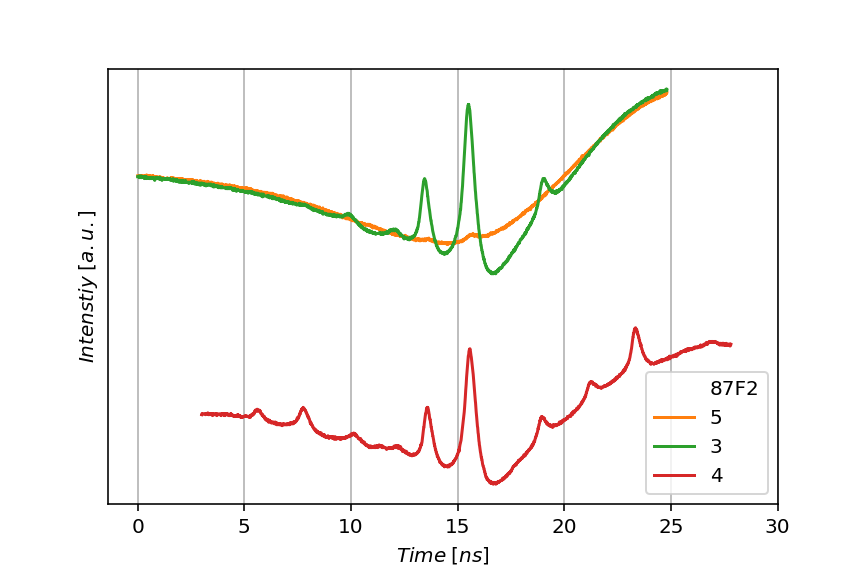
\includegraphics[width=.8\textwidth]{Plots/Calibration_Second_All.png}
\caption{Graphic of the difference between AS and SAS. The hyperfine structure transitions are now visible. In red the SAS while an additional signal generator is on to create the sidebands for calibration purposes.}
\label{fig:all}
\end{figure}

The measurement data taken from the oscilloscope consists of intensities and the time. The orange line for absorption spectroscopy and the green one for saturated AS shifted on top are showing the difference between the methodes.
To determine at which energy a peak is it is necessary to convert the time into an energy or according frequency scale. This is done with the red curve in \autoref{fig:all}. An additional signal generator creates the sidebands in a set frequency distance of $\omega_{shift}=600MHZ$. These sidebands are the difference between green and red curve. They are echoes of the peaks already seen but shifted by $\omega_{shift}/2$ in both directions. Determination of the expected value of each peak in the red curve leads to the conversion rule from time to energy. 

\autoref{fig:calibration} is created by subtracting the AS spectrum from the red curve to increase the visibility of the peaks for better results while fitting them. The fits are Gaussian due to \autoref{eq:gauss} with an error given by the standard derivation $\sigma$. Gaussian function with $\mu$ as expected value:

\begin{equation}
G(x) = A \cdot exp\left( -\frac{(x-\mu)^2}{2\sigma^2} \right)
\end{equation}

\begin{figure}[H]
\centering
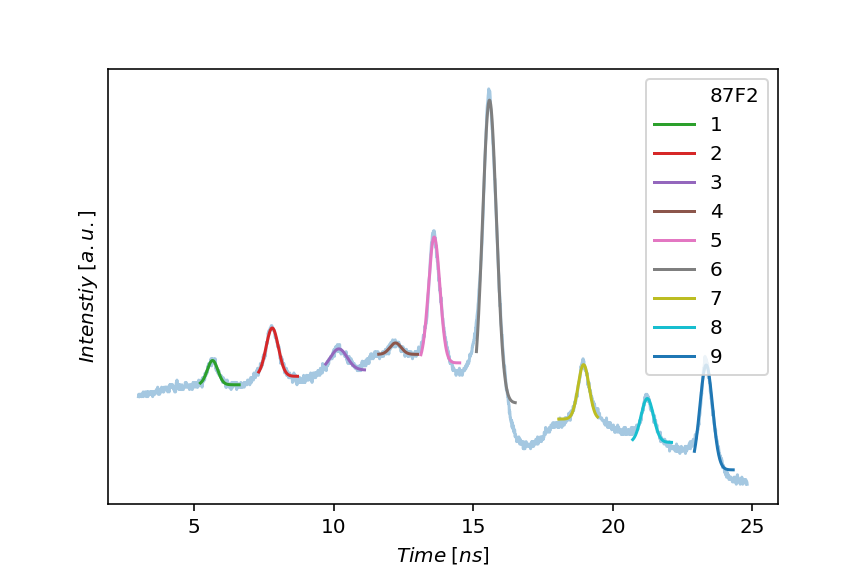
\includegraphics[width=.8\textwidth]{Plots/Calibration_Second_Real.png}
\caption{Saturated absorption spectroscopy with sidebands subtracted with the curve for AS. This improves the visibility of the individual peak. They are already named as shown in the following chapters.}
\label{fig:calibration}
\end{figure}

\begin{table}[H]
\centering
\begin{tabular}{c|c|c}

Peak 1 & Peak 2 & Difference [ns] \\ \hline\hline
SB CO13 left & CO13 & $7.94 \pm 0.28$ \\
CO13 & SB CO13 right & $7.63 \pm 0.31$ \\ \hline 
SB CO23 left & CO23  & $7.78 \pm 0.34$ \\
CO23 & SB CO23 right & $7.75 \pm 0.36$

\end{tabular}
\caption{Time difference between expected values of the peaks as labelled in \autoref{fig:calibration}. The error is given by: $\sqrt{\sigma_1^2 + \sigma_2^2}$.}
\label{tab:calc}
\end{table}

By dividing the equivalent $300\ MHz$ per time difference shown in\autoref{tab:calc} with the average value of $7.78 \pm 0.32\ ns$ results in the following conversion rule.
\begin{equation}
f=t\cdot u \;,\;\; \Delta f = \sqrt{(\Delta t \cdot u)^2+ (t \cdot \Delta u)^2} \;,\;\; u\pm\Delta u= 38.56 \pm 1.59
\label{eq:conversion rule}
\end{equation}


This will now be used to recalibrate the time axis to a scale of frequency. From the relative distance of the peaks we'll be able to identify their origin, by comparing them with the distances given in \autoref{fig:Rb_hyperfine}. 
The relative frequency is determined in comparison with the first named peak and follows \autoref{eq:rel freq}.

\begin{equation}
f_{rel} = f - f_0 \;,\;\; \Delta f_{rel} = \sqrt{ \Delta f^2 + \Delta f_0^2}
\label{eq:rel freq}
\end{equation}


\newpage
\subsection{Rubidium 87, F=2}
\begin{figure}[H]
\centering
\begin{subfigure}{.7\textwidth}
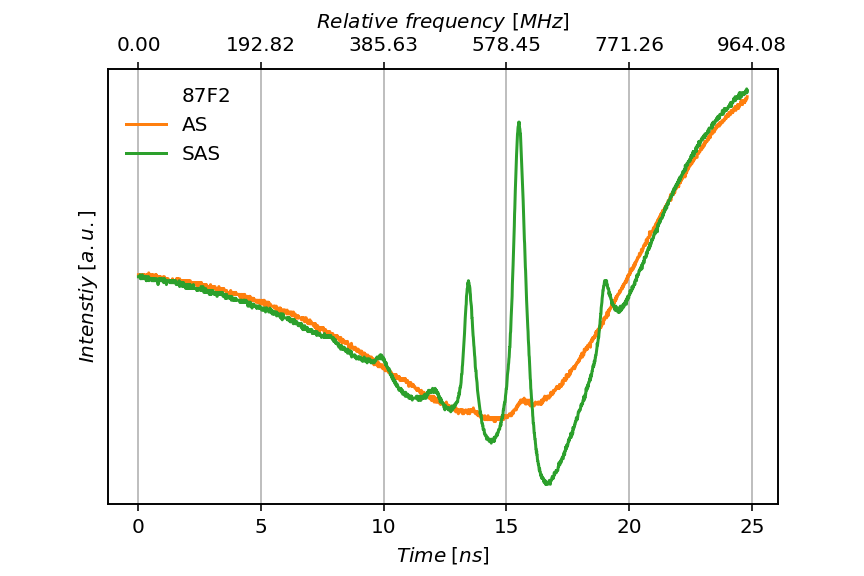
\includegraphics[width=\linewidth]{Plots/87F2_Both.png}
\end{subfigure}

\begin{subfigure}[c]{.7\textwidth}
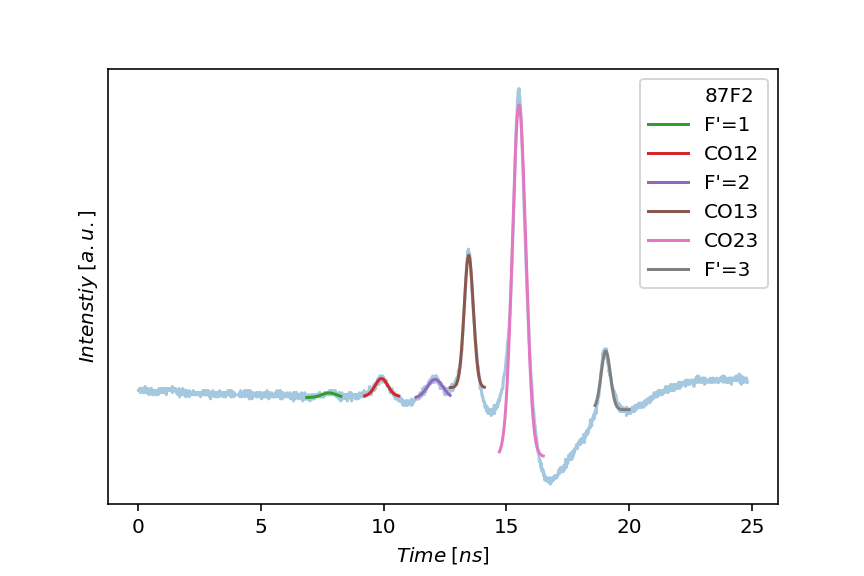
\includegraphics[width=\linewidth]{Plots/87F2_Diff.png}
\end{subfigure}
\caption{$^{87}Rb\ F=2 $. Measured signals on top and difference signal with Gaussian fits for each visible peak underneath.}
\label{fig: 87F2}
\end{figure}

\begin{table}[H]
\centering
\begin{tabular}{|c|c|c|||c|c|}
\hline
Peak & Time $t$ [ns] & Frequency $f$ [MHz] & $f_{rel}$ [MHz] & Name \\ \hline\hline
1 & $7.77 \pm 0.30$  & $299.65 \pm 16.80$  & $0.00 \pm 23.75$  & F'=1 \\ \hline
2 & $9.90 \pm 0.26$  & $381.92 \pm 18.59$  & $82.28 \pm 25.06$  & CO 12 \\ \hline
3 & $12.09 \pm 0.32$  & $466.17 \pm 22.75$  & $166.52 \pm 28.28$  & F'=2 \\ \hline
4 & $13.46 \pm 0.19$  & $519.16 \pm 22.52$  & $219.52 \pm 28.10$  & CO 13 \\ \hline
5 & $15.51 \pm 0.27$  & $598.19 \pm 26.75$  & $298.54 \pm 31.59$  & CO 23 \\ \hline
6 & $19.05 \pm 0.19$  & $734.45 \pm 31.06$  & $434.80 \pm 35.31$  & F'=3 \\ \hline
\hline
\end{tabular}
\caption{$^{87}Rb\ F=2 $. Values for the peaks position and the relative frequency to the first peak allocatable to the spectrum. See \autoref{fig:Rb_hyperfine} and \autoref{tab: rel rb freq}.}
\end{table}

%%% tabel with postional values

\newpage
\subsection{Rubidium 85, F=3}
\begin{figure}[H]
\centering
\begin{subfigure}{.7\textwidth}
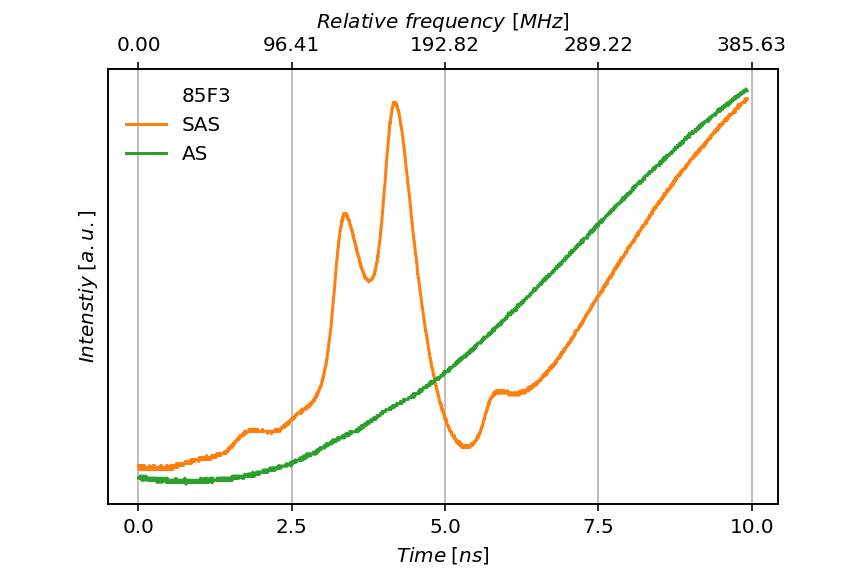
\includegraphics[width=\linewidth]{Plots/85F3_Both.png}
\end{subfigure}

\begin{subfigure}[c]{.7\textwidth}
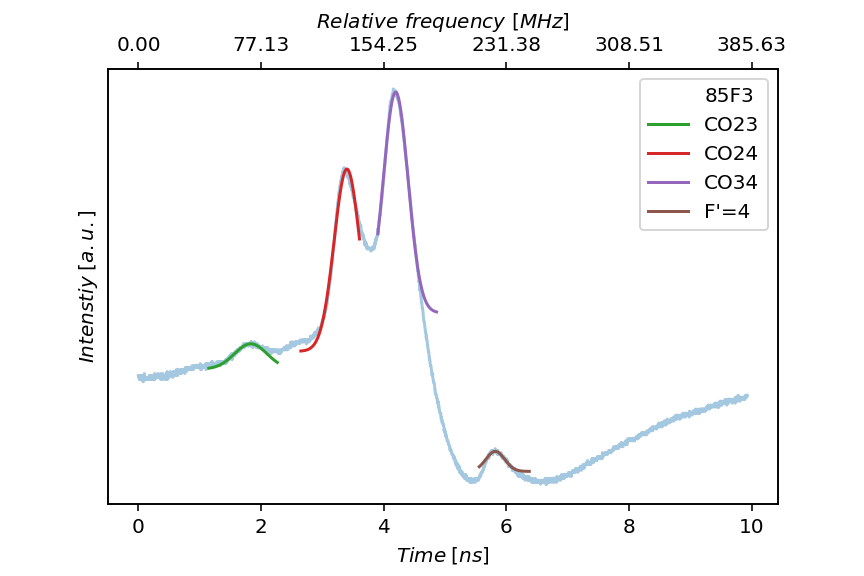
\includegraphics[width=\linewidth]{Plots/85F3_Diff.png}
\end{subfigure}
\caption{$^{85}Rb\ F=3 $. Measured signals on top and difference signal with Gaussian fits for each visible peak underneath.}
\label{fig: 85F3}
\end{figure}

\begin{table}[H]
\centering
\begin{tabular}{|c|c|c|||c|c|}
\hline
Peak & Time $t$ [ns] & Frequency $f$ [MHz] & $f_{rel}$ [MHz] & Name \\ \hline\hline
1 & $1.83 \pm 0.27$  & $70.62 \pm 10.64$  & $0.00 \pm 15.05$  & CO 23 \\ \hline
2 & $3.40 \pm 0.21$  & $131.07 \pm 9.68$  & $60.45 \pm 14.39$  & CO 24 \\ \hline
3 & $4.19 \pm 0.20$  & $161.71 \pm 10.24$  & $91.09 \pm 14.77$  & CO 34 \\ \hline
4 & $5.82 \pm 0.15$  & $224.32 \pm 10.94$  & $153.70 \pm 15.27$  & F'=4 \\ \hline
\hline
\end{tabular}
\caption{$^{85}Rb\ F=3 $. Values for the peaks position and the relative frequency to the first peak allocatable to the spectrum. See \autoref{fig:Rb_hyperfine} and \autoref{tab: rel rb freq}.}
\end{table}


\newpage
\subsection{Rubidium 85, F=2}
\begin{figure}[H]
\centering
\begin{subfigure}{.7\textwidth}
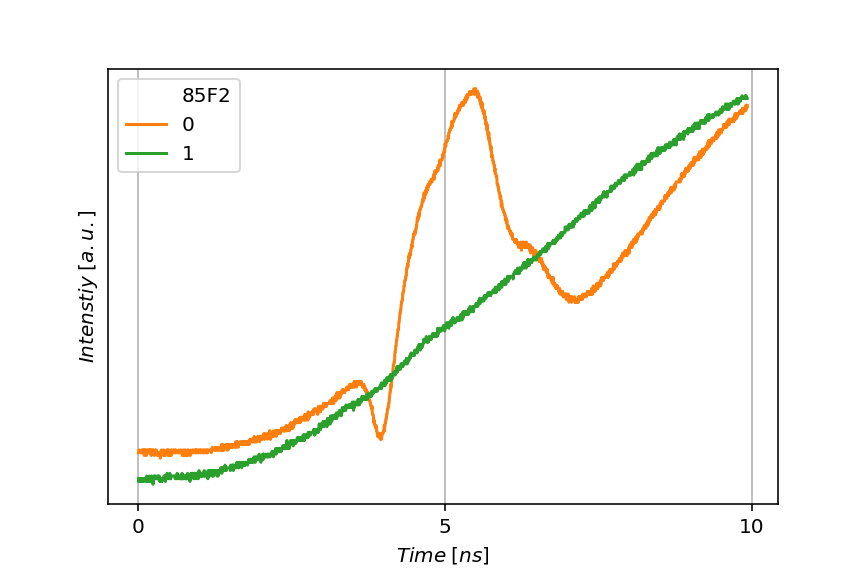
\includegraphics[width=\linewidth]{Plots/85F2_Both.png}
\end{subfigure}

\begin{subfigure}[c]{.7\textwidth}
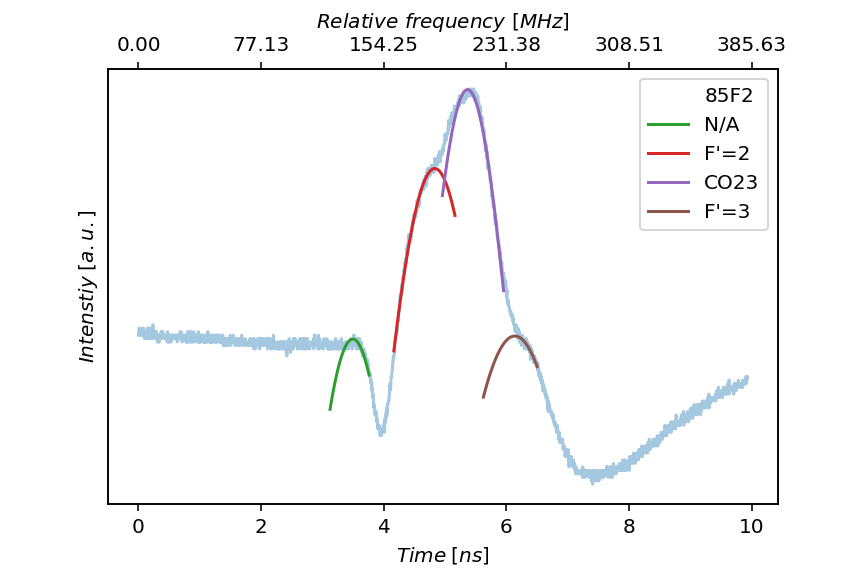
\includegraphics[width=\linewidth]{Plots/85F2_Diff.png}
\end{subfigure}
\caption{$^{85}Rb\ F=2 $. Measured signals on top and difference signal with Gaussian fits for each visible peak underneath.}
\label{fig: 85F2}
\end{figure}

\begin{table}[H]
\centering
\begin{tabular}{|c|c|c|||c|c|}
\hline
Peak & Time $t$ [ns] & Frequency $f$ [MHz] & $f_{rel}$ [MHz] & Name \\ \hline\hline
1 & $3.95 \pm 0.13$  & $152.29 \pm 7.92$  & $-32.90 \pm 35.99$  & N/A \\ \hline
2 & $4.80 \pm 0.89$  & $185.19 \pm 35.11$  & $0.00 \pm 49.65$  & F'=2 \\ \hline
3 & $5.37 \pm 0.77$  & $206.93 \pm 30.71$  & $21.74 \pm 46.64$  & CO 23 \\ \hline
4 & $6.23 \pm 0.52$  & $240.16 \pm 22.40$  & $54.97 \pm 41.64$  & F'=3 \\ \hline
\hline
\end{tabular}
\caption{$^{85}Rb\ F=2 $. Values for the peaks position and the relative frequency to the first peak allocatable to the spectrum. See \autoref{fig:Rb_hyperfine} and \autoref{tab: rel rb freq}.}
\end{table}


\newpage
\subsection{Rubidium 87, F=1}
\begin{figure}[H]
\centering
\begin{subfigure}{.7\textwidth}
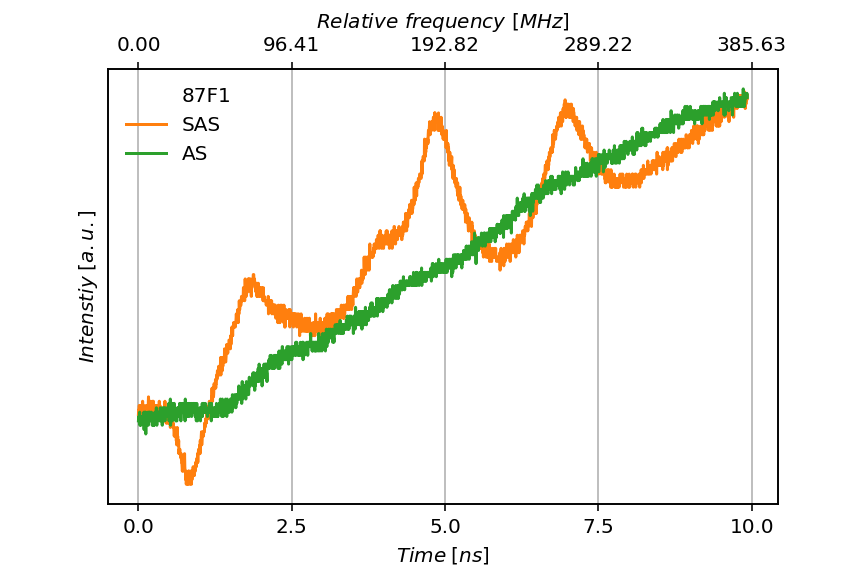
\includegraphics[width=\linewidth]{Plots/87F1_Both.png}
\end{subfigure}

\begin{subfigure}[c]{.7\textwidth}
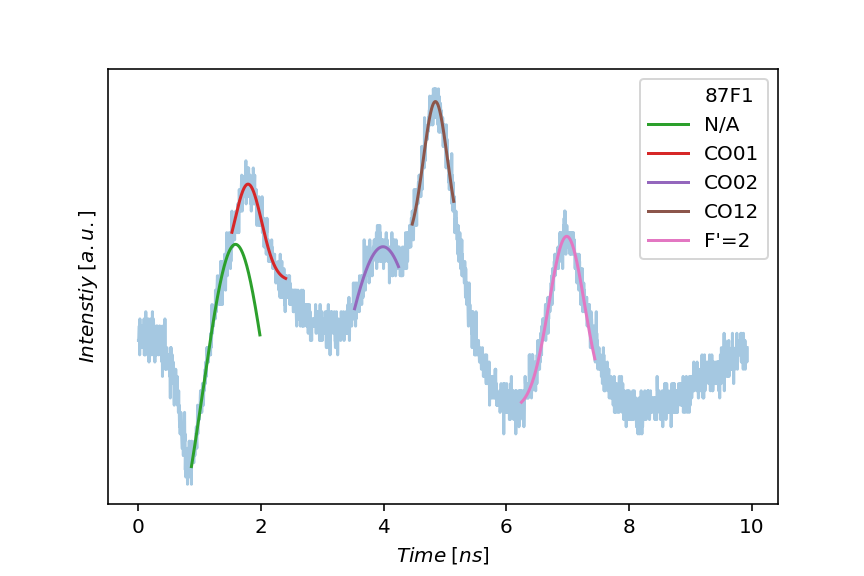
\includegraphics[width=\linewidth]{Plots/87F1_Diff.png}
\end{subfigure}
\caption{$^{87}Rb\ F=1 $. Measured signals on top and difference signal with Gaussian fits for each visible peak underneath.}
\label{fig: 87F1}
\end{figure}

\begin{table}[H]
\centering
\begin{tabular}{|c|c|c|||c|c|}
\hline
Peak & Time $t$ [ns] & Frequency $f$ [MHz] & $f_{rel}$ [MHz] & Name \\ \hline\hline
1 & $1.58 \pm 0.53$  & $61.03 \pm 20.59$  & $-7.87 \pm 22.50$  & N/A \\ \hline
2 & $1.79 \pm 0.22$  & $68.90 \pm 9.07$  & $0.00 \pm 12.83$  & CO 01 \\ \hline
3 & $3.99 \pm 0.70$  & $153.76 \pm 27.78$  & $84.85 \pm 29.23$  & CO 02 \\ \hline
4 & $4.84 \pm 0.20$  & $186.71 \pm 10.76$  & $117.80 \pm 14.08$  & CO 12 \\ \hline
5 & $6.98 \pm 0.29$  & $269.25 \pm 15.78$  & $200.35 \pm 18.20$  & F'=2 \\ \hline
\hline
\end{tabular}
\caption{$^{87}Rb\ F=1 $. Values for the peaks position and the relative frequency to the first peak allocatable to the spectrum. See \autoref{fig:Rb_hyperfine}.}
\end{table}


\newpage
\subsection{Temperature estimation of Rubidium}
To estimate the temperature of the rubidium gas the Doppler broadening seen in \autoref{fig:signals} has to be fitted with two different Gaussians for higher precision. One on the right and one on the left side to receive a value for the FWHM, as shown in \autoref{fig:Doppler whole broken}.

\begin{figure}[H]
\centering
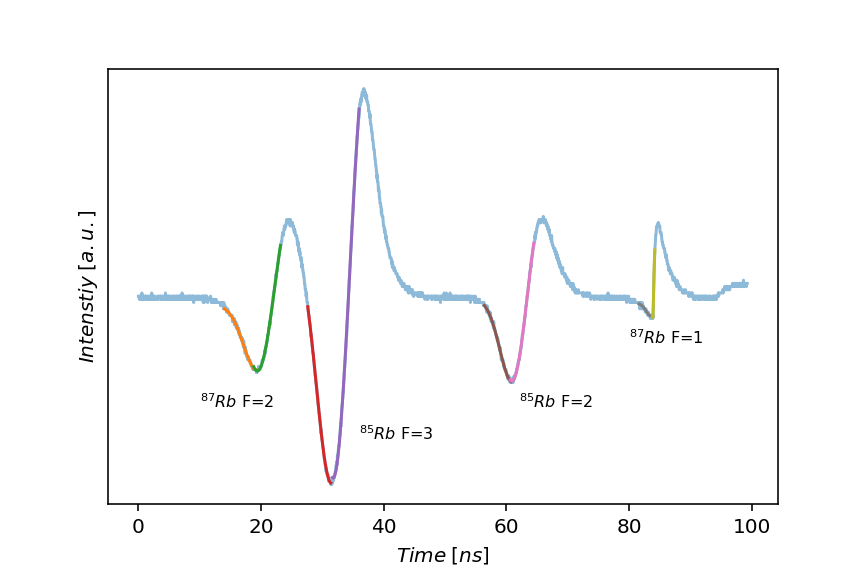
\includegraphics[width=.9\textwidth]{Plots/Doppler_whole.png}
\caption{Doppler broadening spectrum. Each side of a transitions peak is fitted separately with a Gaussian to determine the FWHM.}
\label{fig:Doppler whole broken}
\end{figure}

To calculate the Doppler width $\delta v_D$ the double standard derivation of the Gaussians mean value is used. Because there are two slightly different fits on each peaks side, the mean value of them will be calculated. This is shown in \autoref{tab:wrong temps} column Time $2\sigma_t$. The calculation is given by:

\begin{equation}
\sigma_t = \frac{1}{2}\cdot(\sigma_{left} + \sigma_{right}) \;,\quad \Delta\sigma_t = \frac{1}{2} \cdot |\sigma_{left} - \sigma_{right}|
\end{equation}

We are using \autoref{eq:gauss} to create the connection between FWHM and the gas temperature. We will use the Doppler width $\delta v_D = \delta \omega_D /2\pi$ as FWHM, because we are comparing the values with the transition frequencies. By rewriting the equation and inserting $c=\lambda_0 \cdot \omega_0 /2\pi$ we get the following equation:

\begin{gather}
\delta v_D = \frac{2}{2\pi}\ \sqrt{ln(2)}\  \frac{2\pi}{\lambda_0}\ \sqrt{\frac{2k_BT}{m}} \\
T = \frac{m}{8ln(2)k_B}\ \lambda_0^2 \cdot \delta v_D^2\ =:\ k \cdot\delta v_D^2 \;,\;\; \Delta T = k \cdot 2\delta v_D \Delta\delta v_D
\end{gather}

The problem with \autoref{fig:Doppler whole broken} is that this spectrum was taken for an other calibration and therefore useless for our determination of the temperature. We missed taking another complete Doppler broadening spectrum.
The values for the four peaks shown here are presented in\autoref{tab:wrong temps}.

\begin{table}[H]
\centering
\begin{tabular}{|c|c|c|c|}
\hline
Peak & Time $2\sigma_t\ [ns]$ & $\delta v_D\ [MHz]$ & Temperature $[K]$ \\ \hline\hline
$^{87}Rb$ F=2 & $6.00 \pm 0.77$  & $231.42 \pm 31.31$  & $60.07 \pm 16.26$  \\ \hline
$^{85}Rb$ F=3 & $6.12 \pm 0.33$  & $235.97 \pm 16.12$  & $62.45 \pm 8.53$  \\ \hline
$^{85}Rb$ F=2 & $5.43 \pm 0.63$  & $209.53 \pm 25.93$  & $49.24 \pm 12.19$  \\ \hline
$^{87}Rb$ F=1 & $1.18 \pm 0.82$  & $45.57 \pm 31.55$  & $2.33 \pm 3.23$  \\ \hline
\hline
\end{tabular}
\caption{Calculated values for the $\delta v_D$ as the FWHM mean value for each peak and the according Temperature.}
\label{tab:wrong temps}
\end{table}

The expected Temperature was displayed at the lasers configuration panel. Over the course of the experiment the value was steadily $20.4^\circ C = 297.55 K$, which is the average room temperature. This is not directly the temperature of the rubidium gas. The tansversing light will increase its temperature and therefore we assumed a temperature of about $300K$. Comparing this to the upper values, the argumentation of a different calibration is valid, although the last peaks fit should be excluded due to an insufficient amount of data values taken.

Luckily the spectrum of $^{87}Rb\ F=2$ provided the possibility to fit both sides of the Doppler broadening. The results are presented in \autoref{fig:Doppler 87F2 good}.

\begin{figure}[H]
\centering
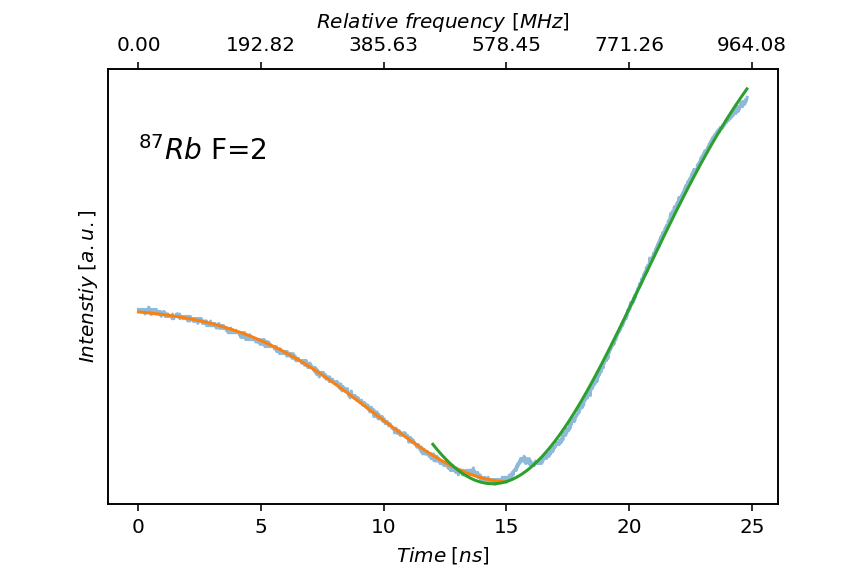
\includegraphics[width=.8\textwidth]{Plots/Doppler_87F2.png}
\caption{Fits for the Doppler width at the example of the Doppler broadening peak $^{87}Rb\ F=2$.}
\label{fig:Doppler 87F2 good}
\end{figure}

\begin{table}[H]
\centering
\begin{tabular}{|c|c|c|c|}
\hline
Peak & Time $2\sigma_t\ [ns]$ & $\delta v_D\ [MHz]$ & Temperature $[K]$ \\ \hline\hline
$^{87}Rb$ F=2 & $13.82 \pm 0.62$  & $533.13 \pm 32.43$ & $318.80 \pm 38.67$   \\ \hline
\hline
\end{tabular}
\end{table}

This temperature is a good value compared to the others. Its error is covering a broad range and without any other values for comparison this is not a good result. But the method stays the same and with more values a mean value could have shown a lower temperature which we expected. Gas temperatures much higher than the average room temperature would be unrealistic, due to thermal heat transfer provided by the glass walls of the gas cell.

\subsection{Error analysis}
Most of the errors are given by the standard derivation of Gaussian fits. This value is used, because the error on the expected value $\mu$ is very low to good fitting data values. This ensures that influences like slightly shifting laser current and fluctuations in the signal generator frequency are covered.

We tried to arrange the mirrors for the maximum overlap of the tow laser beams, but less overlap effects directly the intensity and thereby the quality of our fits. But a perfect overlapping laser path was not possible.

The choice of the right laser current was also important. This affected the quality of the peaks registered. In the beginning we had a good current, but somehow the signal was lost and we had to calibrate again. This is where the difference in the temperature estimation comes from.


\subsection{Discussion}
Returning to the identification of the hyperfine transitions the naming of the peaks was done by comparing the relative values in \autoref{tab: rel rb freq}. Worth mentioning is that the cross over peaks are mostly the higher ones, due to the excitation of two different energy levels. Therefore this is a good starting point for comparison. For $^{85}Rb\ F=2$ and $^{87}Rb\ F=1$ the first peak is labelled "N/A" which should suggest that there is no real peak. This is an artefact of the first attempts to see many transitions. But in the end they are none, although in some graphics one could think of them as a peak. Therefore their values from the relative frequency calculation are regardless.

The best result is the $^{87}Rb\ F=2$ graphic where all transitions are found. With increasing transition energy from $5^2S_{1/2} \rightarrow 5^2P_{3/2}$ the quality gets lower, although the graphics for $^{87}Rb$ are in general from better quality, due to the higher energy distance in the $5^2P_{3/2}$ state. Interesting is that the ratio of $^{87}Rb$ and $^{85}Rb$ doesn't influence the quality regarding to more atoms results in a better resolution of the peaks.

We took additional data to see the effects of the Zeeman effect, but the effects on the oscilloscope were poorly and the analysis would have taken too much additional time, which was needed for the following experiment, which is funnily enough the Zeeman effect.



\newpage
\section{Conclusion}
The results of this experiment are satisfying but not extraordinary good. The calibration worked as expected, but with an additional peak in the sidebands the value could have been more precise. We have not been able to display all of the possible hyperfine transitions and cross over peaks, but at least there were 50\% of them visible and matchable. The first $^{87}Rb\ F=2$ spectrum contains actually all of the peak. Positive is that the relative frequency to the first peak is most of the time pretty accurate. Within the errors given, the values are showing the expected hyperfine structure for at least $^{87}Rb$.

As shown the application of saturated absorption spectroscopy instead of the usual one increases the resolving capacity of the transitions dramatically. Laser spectroscopy is a good way to analyse the energy structure of chemical elements and to confirm quantum mechanical effects like the hyperfine structure.



\section{Appendix}
\subsection{Rubidiums hyperfine structure}
\begin{figure}[H]
\centering
\begin{subfigure}{.8\textwidth}
\centering
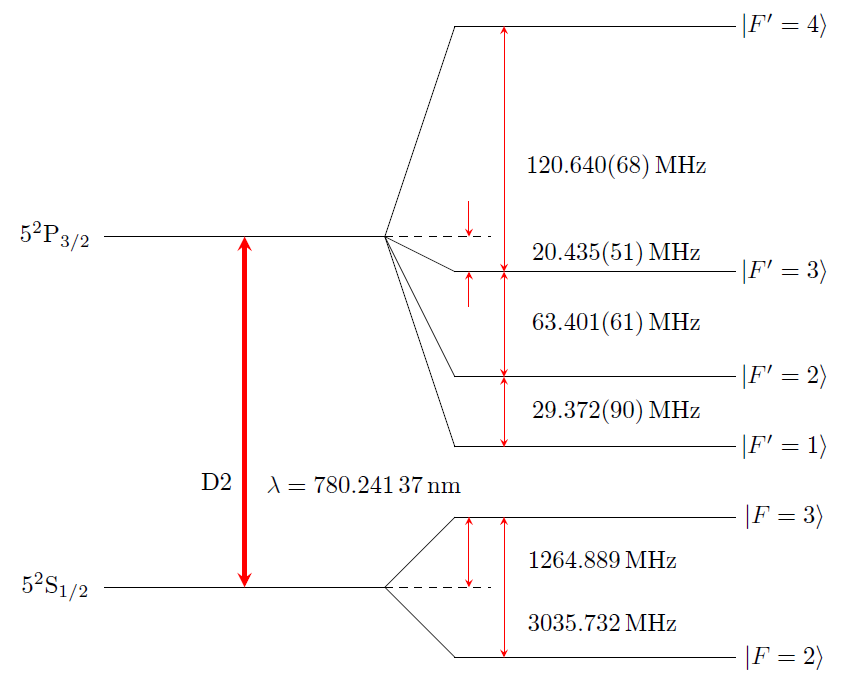
\includegraphics[width=1\textwidth]{Plots/Level85.png}
\caption{Hyperfine structure of Rubidium 85 \cite{steck85} }
\end{subfigure}

\begin{subfigure}{.8\textwidth}
\centering
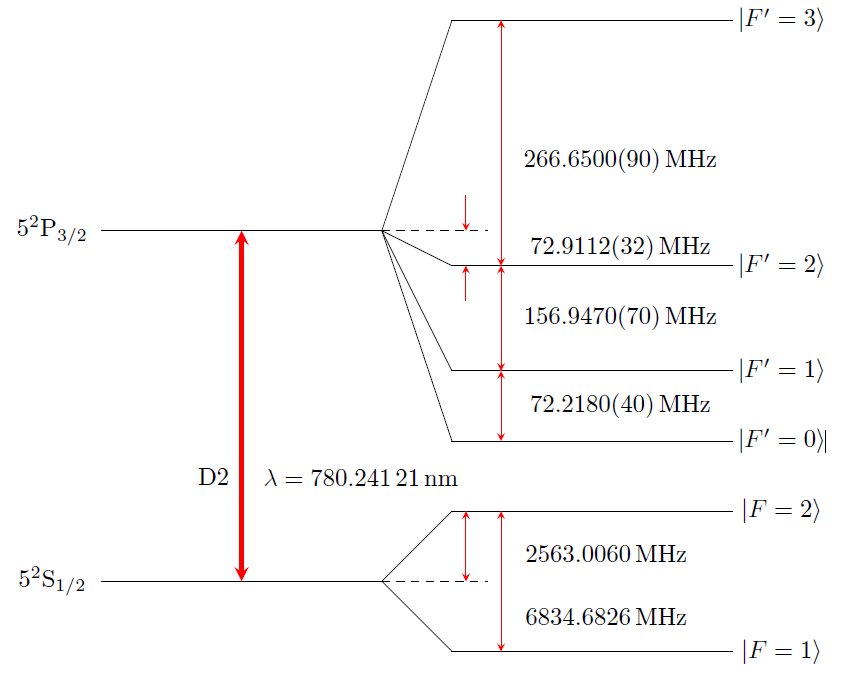
\includegraphics[width=1\textwidth]{Plots/Level87.png}
\caption{Hyperfine structure of Rubidium 87 \cite{steck87}}
\end{subfigure}

\caption{Hyperfine structure of both used rubidium isotopes.}
\label{fig:Rb_hyperfine}
\end{figure}

\begin{table}[H]
\centering
\begin{tabular}{c|c|c| |c|c|c}
$^{85}Rb$ & F=2 & F=3 & $^{87}Rb$ & F=1 & F=2 \\ \hline\hline
F'=1 & 0    & -     & F'=0 & 0     & - \\
CO 12& 14.69& -     & CO 01& 36.11 & - \\
F'=2 & 29.37& 0     & F'=1 & 72.22 & 0 \\
CO 13& 46.39& -     & CO 02& 114.59& - \\
CO 23& 61.07& 31.70 & CO 12& 150.70& 78.48 \\
F'=3 & 92.77& 63.40 & F'=2 & 229.17& 156.95 \\
CO 24& -    & 92.02 & CO 13& -     & 211.80 \\
CO 34& -    & 123.72& CO 23& -     & 280.28 \\
F'=4 & -    & 184.04& F'=3 & -     & 423.60 \\
\end{tabular}
\caption{Expected frequency differences [MHz] for the four hyperfine transitions relative to the lowest possible one. Given by \autoref{fig:Rb_hyperfine} and \autoref{tab: rel rb freq}.}
\label{tab: rel rb freq}
\end{table}


\newpage
\begin{thebibliography}{}
\bibitem[Steck85]{steck85} Rubidium 85 D Line Data, Daniel Adam Steck, University of Oregon

\bibitem[Steck87]{steck87} Rubidium 87 D Line Data, Daniel Adam Steck, University of Oregon

\bibitem[Dem3]{dem3} Demtröder Experimentalphysik 3: Atome, Moleküle und Festkörper, Springer


\end{thebibliography}
\end{document}

